\section{SHAP robustness under augmentation}\label{sec:stability}

Although augmentation did not improve prediction, it provides a useful perturbation test: if
the descriptor hierarchy survives having the training set resampled from a learned Bayesian
network, it is not an artefact of the particular rows sampled.

Comparing the cohort real-only model with the best-performing augmented model on the identical
cohort and feature set (Fig.~\ref{fig:stab}):

\begin{itemize}
\item Spearman rank correlation of descriptor rankings:
$\rho = 0.90$ ($p = 0.037$).
\item Top-3 overlap 3/3; top-5 overlap 5/5.
\item Mean absolute rank displacement 0.4 positions
(maximum 1).
\item Mean absolute change in each descriptor's share of total attribution:
0.018.
\end{itemize}

The descriptor hierarchy is therefore stable. This matters for the argument of this paper: the
same experiment that fails to improve prediction succeeds in demonstrating that the
\emph{relative} descriptor ordering is robust to resampling of the training distribution.
Had augmentation improved $R^2$ while substantially reordering the descriptors, that would
have indicated synthetic-distribution distortion and the ranking would not be usable; the
observed combination --- no predictive gain, high attribution stability --- is the one that
licenses using the real-only SHAP ranking for descriptor selection.

\begin{figure*}[htbp]\centering
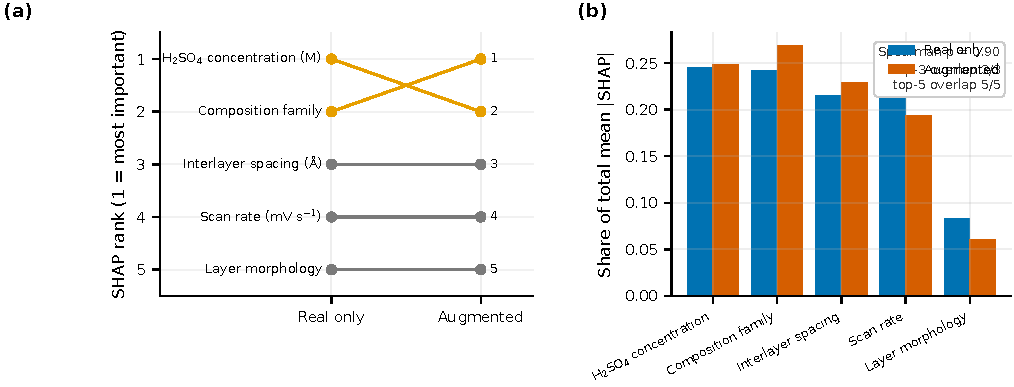
\includegraphics[width=\textwidth]{figures/fig08_shap_stability.pdf}
\caption{Descriptor attribution before and after Bayesian augmentation. (a) Rank slope chart;
grey lines indicate unchanged rank. (b) Share of total mean $|$SHAP$|$ per descriptor.}
\label{fig:stab}\end{figure*}
